\documentclass[usenames,dvipsnames,aspectratio=169]{beamer}
\usepackage{../common/prgBasics}
\usepackage{tabularx}

\title[Lecture 4.]{Programming basics}
\subtitle{(GKNB\_INTA023)}

\begin{document}

%1
\begin{frame}[plain]
  \titlepage
  \logoalul
\end{frame}

%2
\begin{frame}{Triangle equality}
  \begin{exampleblock}{\textattachfile{triangle1.c}{triangle1.c} ANSI C (C89) compliant implementation}
  \tiny
  \vspace{-.3cm}
  \lstinputlisting[style=c]{triangle1.c}
  \vspace{-.3cm}
  \end{exampleblock}
\end{frame}

%3
\begin{frame}{Triangle equality}
  \footnotesize
  \begin{exampleblock}{\textattachfile{triangle2.c}{triangle2.c} C99 compliant implementation; reading side lengths are repeated 3x!}
  \tiny
  \vspace{-.3cm}
  \lstinputlisting[style=c]{triangle2.c}
  \vspace{-.3cm}
  \end{exampleblock}
\end{frame}

%4
\begin{frame}{Triangle equality}
  \begin{exampleblock}{\textattachfile{triangle3.c}{triangle3.c}}
    \tiny
    \vspace{-.3cm}
    \lstinputlisting[style=c]{triangle3.c}
    \vspace{-.3cm}
  \end{exampleblock}
\end{frame}

%5
\begin{frame}[fragile]{Triangle equality}
  Array definition
  \begin{itemize}
    \item \emph{type name[size];}
    \item eg. \texttt{int sideArray[3];}
    \item \emph{size} is a positive integer valued \emph{constant expression}
    \item the value of a \emph{constant expression} can be calculated compile-time
  \end{itemize}
  Memory requirement of an array
  \begin{itemize}
    \item[] \emph{sizeof(name\_of\_the\_array) $\equiv$ size*sizeof(type)}
  \end{itemize}
  Accessing array elements
  \begin{itemize}
    \item \emph{name[index]}
    \item 0 $\leq$ \emph{index} $\leq$ \emph{size}$-$1
  \end{itemize}
  \hspace{4mm}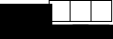
\includegraphics[]{array.pdf}
\end{frame}

%6
\begin{frame}{Triangle equality}
    \begin{exampleblock}{\textattachfile{triangle4.c}{triangle4.c}}
    \tiny
    \vspace{-.3cm}
    \lstinputlisting[style=c]{triangle4.c}
    \vspace{-.3cm}
  \end{exampleblock}
\end{frame}

%7
\begin{frame}[fragile]{Triangle equality}
  Generating side names
  \begin{itemize}
    \item ASCII codes of letters in ascending order are also increasing \\ ('A' == 65, 'B' == 66, 
\dots, 'Z' == 90)
    \item Digits are encoded similarly ('0' == 48, '1' == 49, \dots, '9' == 57)
    \item Digit $\rightarrow$ ASCII code: \texttt{'0'+digit}
    \item ASCII code $\rightarrow$ digit: \texttt{character-'0'}
    \item Letters can be handled similarly
  \end{itemize}
  \begin{exampleblock}{}
    \tiny
    \lstinputlisting[style=c,linerange={14-14},firstnumber=14]{triangle4.c}
  \end{exampleblock}
  Format specifier: \kiemel{\texttt{\%c}} (single character, not terminated by zero!)\\
  Character literals are between apostrophes!
\end{frame}

%8
\begin{frame}{Counting digits}
    \begin{exampleblock}{\textattachfile{counter1.c}{counter1.c} 1/2}
    \tiny
    \lstinputlisting[style=c,lastline=23]{counter1.c}
  \end{exampleblock}
\end{frame}

%9
\begin{frame}{Counting digits}
    \begin{exampleblock}{\textattachfile{counter1.c}{counter1.c} 2/2}
    \scriptsize
    \lstinputlisting[style=c,firstline=24,firstnumber=24]{counter1.c}
  \end{exampleblock}
  \vfill
  We urgently need an array!
\end{frame}

%10
\begin{frame}{Counting digits}
    \begin{exampleblock}{\textattachfile{counter2.c}{counter2.c} 1/2}
    \footnotesize
    \lstinputlisting[style=c,lastline=13]{counter2.c}
  \end{exampleblock}
\end{frame}

%11
\begin{frame}{Counting digits}
    \begin{exampleblock}{\textattachfile{counter2.c}{counter2.c} 2/2}
    \scriptsize
    \lstinputlisting[style=c,firstline=14,firstnumber=15]{counter2.c}
  \end{exampleblock}
\end{frame}

%12
\begin{frame}{Counting digits}
  Array elements as counters
  \begin{itemize}
    \item[] The quantity of digit \kiemel{i} is stored at \kiemel{digits[i]} (eg. 0 $\to$ digits[0], 1 $\to$ digits[1], etc.)
  \end{itemize}
  \vfill
  Initialization of arrays
  \begin{itemize}
    \item \emph{type name[<size>]<={initializer\_list}>;}
    \item If the number of elements in \emph{initializer\_list} $<$ \emph{size} $\to$ remaining elements are reset to zero
    \item If the number of elements in \emph{initializer\_list} $>$ \emph{size} $\to$ ERROR!
    \item If \emph{size} is not specified, the compiler counts the elements of \emph{initializer\_list}
    \item But at least one of \emph{size} and \emph{initializer\_list} must exist!
  \end{itemize}
\end{frame}

%13
\begin{frame}{Counting digits}
    \begin{exampleblock}{\textattachfile{counter3.c}{counter3.c}}
    \tiny
    \lstinputlisting[style=c]{counter3.c}
  \end{exampleblock}
\end{frame}

%14
\begin{frame}{Printing numbers in reverse order}
    \begin{exampleblock}{\textattachfile{reverse1.c}{reverse1.c}}
    \fontsize{8}{9} \selectfont
    \lstinputlisting[style=c]{reverse1.c}
  \end{exampleblock}
\end{frame}

%15
\begin{frame}{Printing numbers in reverse order}
    \begin{exampleblock}{\textattachfile{reverse2.c}{reverse2.c}}
    \scriptsize
    \lstinputlisting[style=c]{reverse2.c}
  \end{exampleblock}
\end{frame}

%16
\begin{frame}{Linear (sequential, serial) search}
    \begin{exampleblock}{\textattachfile{sequential.c}{sequential.c} ($\to$ \href{https://en.wikipedia.org/wiki/Linear\_search}{Linear search})}
    \scriptsize
    \lstinputlisting[style=c]{sequential.c}
  \end{exampleblock}
\end{frame}

%17
\newcommand{\mc}[3]{\multicolumn{#1}{#2}{#3}}
\begin{frame}{Binary search}
  \hiv{\href{https://en.wikipedia.org/wiki/Binary\_search\_algorithm}{Binary search}} can be used only with ordered arrays!
  \vfill
  \begin{columns}[c]
    \column{0.5\textwidth}
      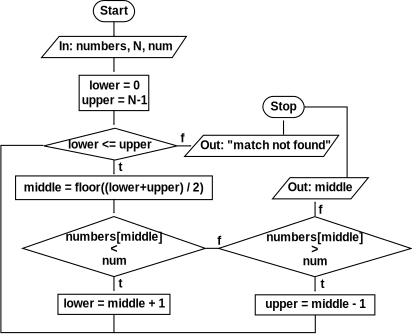
\includegraphics[width=\textwidth]{binary.pdf}
    \column{0.5\textwidth}
    {
      \footnotesize
      \setlength\tabcolsep{1.5pt}
      \begin{tabularx}{\linewidth}{*{10}{>{\centering\arraybackslash}X}}
      \mc{10}{l}{numbers}\\\hline
      \mc{1}{|c|}{-23} & \mc{1}{c|}{-11} & \mc{1}{c|}{0} & \mc{1}{c|}{1} & \mc{1}{c|}{7} & \mc{1}{c|}{13} & \mc{1}{c|}{14} & 
      \mc{1}{c|}{17} & \mc{1}{c|}{21} & \mc{1}{c|}{42}\\\hline
      0 & 1 & 2 & 3 & 4 & 5 & 6 & 7 & 8 & 9
      \end{tabularx}
      \begin{tabular}{c}
      num\\\hline
      \mc{1}{|c|}{1}\\\hline
      \end{tabular}
      \\\smallskip 
      \begin{tabular}{l|ccc}
        & \texttt{lower} & \texttt{middle}& \texttt{upper} \\\hline
      1 & \kiemel{0}    & ?             & \kiemel{9} \\
      2 & 0             & \kiemel{4}    & 9 \\
      3 & 0             & 4             & \kiemel{3} \\
      4 & 0             & \kiemel{1}    & 3 \\
      5 & \kiemel{2}    & 1             & 3 \\
      6 & 2             & \kiemel{2}    & 3 \\
      7 & \kiemel{3}    & 2             & 3 \\
      8 & 3             & \kiemel{3}    & 3 \\
      \end{tabular}
    }
  \end{columns}
\end{frame}

%18
\begin{frame}{Binary search}
  \begin{exampleblock}{\textattachfile{binary.c}{binary.c}}
    %\tiny
    \vspace{-.3cm}
    \fontsize{7}{8} \selectfont
    \lstinputlisting[style=c]{binary.c}
    \vspace{-.3cm}
  \end{exampleblock}
\end{frame}

%19
\begin{frame}{Bubble sort}
  \begin{center}
    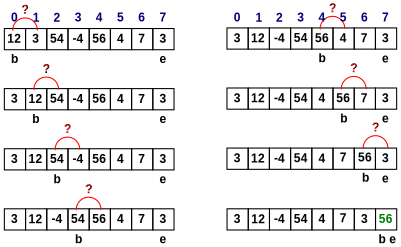
\includegraphics[scale=.9]{bubble_animation1.pdf}
  \end{center}
\end{frame}

%20
\begin{frame}{Bubble sort}
  \begin{center}
    \includegraphics[scale=.9]{bubble_animation2.pdf}
  \end{center}
\end{frame}

%21
\begin{frame}{Bubble sort}
  \begin{center}
    \includegraphics[scale=.9]{bubble_animation3.pdf}
  \end{center}
\end{frame}

%22
\begin{frame}{Bubble sort}
  \begin{center}
    \includegraphics[scale=.9]{bubble_animation4.pdf}
  \end{center}
\end{frame}

%23
\begin{frame}{Bubble sort}
  \begin{center}
    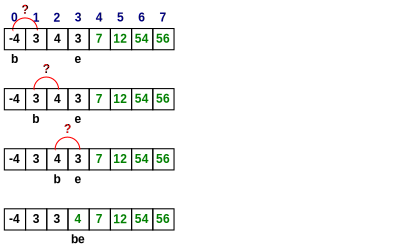
\includegraphics[scale=.9]{bubble_animation5.pdf}
  \end{center}
\end{frame}

%24
\begin{frame}{Bubble sort}
  \begin{center}
    \includegraphics[scale=.9]{bubble_animation6.pdf}
  \end{center}
\end{frame}

%25
\begin{frame}{Bubble sort}
  \begin{center}
    \includegraphics[scale=.9]{bubble_animation7.pdf}
  \end{center}
\end{frame}

%26
\begin{frame}{Bubble sort}
  \begin{center}
    \includegraphics[scale=.9]{bubble_animation8.pdf}
  \end{center}
\end{frame}

%27
\begin{frame}{Bubble sort}
  \begin{center}
    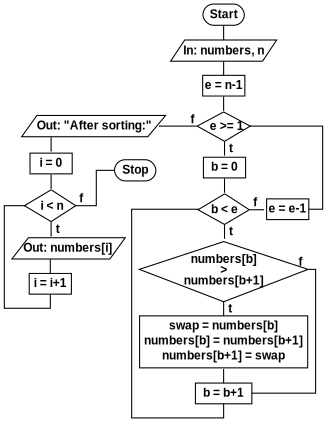
\includegraphics[scale=0.55]{bubble.pdf}
  \end{center}
\end{frame}

%28
\begin{frame}{Bubble sort}
  \begin{exampleblock}{\textattachfile{bubble.c}{bubble.c} ($\to$ \href{https://en.wikipedia.org/wiki/Bubble\_sort}{Bubble sort})}
    \tiny
    \vspace{-.3cm}
    \lstinputlisting[style=c]{bubble.c}
    \vspace{-.3cm}
  \end{exampleblock}
\end{frame}

%29
\begin{frame}{Basics of string handling}
  \kiemel{No type} in C for strings! $\to$ character arrays terminated by the null character (\texttt{'\textbackslash 
0'})\\
  \vfill
  \begin{tabular}{cccccc}
    & 0 & 1 & 2 & 3 & 4 \\\cline{2-6}
    \mc{1}{c|}{s} & \mc{1}{c|}{J} & \mc{1}{c|}{a} & \mc{1}{c|}{n} & \mc{1}{c|}{e} & \mc{1}{c|}{'\textbackslash 0'} \\\cline{2-6}
  \end{tabular}
  \vfill
  String manipulation with functions, eg.
  \begin{description}[mm]
    \item[\texttt{strcat}]\hfill\\ Concatenates (appends) the content of the second string with the first
    \item[\texttt{strcpy}]\hfill\\ Copies the content of the second string in the first one
    \item[\texttt{strlen}]\hfill\\ Determines the length of the string (without the \texttt{'\textbackslash 0'} character)
    \item[\texttt{strcmp}]\hfill\\ Compares the content of strings (based on ASCII codes)
  \end{description}
  Required header: \kiemel{\texttt{string.h}}
\end{frame}

%30
\begin{frame}{Basics of string handling}
  \begin{exampleblock}{\textattachfile{string.c}{string.c}}
    \scriptsize
    \lstinputlisting[style=c,lastline=16]{string.c}
  \end{exampleblock}
\end{frame}

%31
\begin{frame}{Basics of string handling}
  \begin{exampleblock}{\textattachfile{string.c}{string.c}}
    \scriptsize
    \lstinputlisting[style=c,firstline=17,firstnumber=17]{string.c}
  \end{exampleblock}
\end{frame}

%32
\begin{frame}[fragile]{Basics of string handling}
  \begin{block}{Output}
    \begin{verbatim}
Title of the tale: Tom and Jerry
Title length: 13
Memory needed: 128 bytes.
Another tale: The Flinstones
Not funny: The Gerry
The follows Gerry.
\end{verbatim}
  \end{block}
\end{frame}

%33
\begin{frame}{Converting binary numbers to decimals}
  \begin{exampleblock}{\textattachfile{bintodec.c}{bintodec.c}}
    \scriptsize
    \lstinputlisting[style=c]{bintodec.c}
  \end{exampleblock}
\end{frame}

%34
\begin{frame}{Converting decimal numbers to binary}
  \begin{exampleblock}{\textattachfile{dectobin.c}{dectobin.c}}
    \scriptsize
    \vspace{-.3cm}
    \lstinputlisting[style=c]{dectobin.c}
    \vspace{-.3cm}
  \end{exampleblock}
\end{frame}

%35
\begin{frame}{Checking Neptun code}
  \begin{exampleblock}{\textattachfile{neptun1.c}{neptun1.c}}
    \tiny
    \vspace{-.3cm}
    \lstinputlisting[style=c]{neptun1.c}
    \vspace{-.3cm}
  \end{exampleblock}
\end{frame}

%36
\begin{frame}{Checking Neptun code}
    \begin{exampleblock}{\textattachfile{neptun2.c}{neptun2.c}}
    \tiny
    \vspace{-.3cm}
    \lstinputlisting[style=c]{neptun2.c}
    \vspace{-.3cm}
  \end{exampleblock}
\end{frame}

%37
\begin{frame}{Checking Neptun code}
  Classification and conversion of characters
  \begin{itemize}
    \item \texttt{ctype.h} must be included
    \item May be implemented by functions or macros (preprocessor)
    \item The type of parameter is \texttt{int}, but the values must be representable by an \texttt{unsigned char} or \texttt{EOF}
    \item The return value is \texttt{int}, consider as logical value
  \end{itemize}
  \footnotesize
  \begin{center}
    \begin{tabular}{ll}
    Fn./macro name & Goal\\ \hline
    \texttt{islower(c)} & is \texttt{c} a lowercase letter?\\
    \texttt{isupper(c)} & is \texttt{c} an uppercase letter?\\
    \texttt{isalpha(c)} & is \texttt{c} a letter?\\
    \texttt{isdigit(c)} & is \texttt{c} a digit?\\
    \texttt{isalnum(c)} & is \texttt{c} alphanumeric?\\
    \texttt{isxdigit(c)} & is \texttt{c} a hexadecimal digit?\\
    \texttt{isspace(c)} & is \texttt{c} whitespace?\\
    \texttt{isprint(c)} & can\texttt{c} be printed?\\
    \texttt{tolower(c)} & lowercase version of \texttt{c} if \texttt{c} is an uppercase letter\\
    \texttt{toupper(c)} & uppercase version of \texttt{c} if \texttt{c} is a lowercase letter
    \end{tabular}
  \end{center}
\end{frame}

%38
\begin{frame}{Checking Neptun code}
    \begin{exampleblock}{\textattachfile{neptun3.c}{neptun3.c}}
    \tiny
    \lstinputlisting[style=c]{neptun3.c}
  \end{exampleblock}
\end{frame}

\end{document}
